\documentclass[xcolor=dvipsnames]{beamer}
\usepackage[english]{babel}
\usepackage[utf8]{inputenc}

\usepackage{xkeyval}
%\usepackage{todonotes}
%\presetkeys{todonotes}{inline}{}
\usepackage{dsfont}
\usepackage{verbatim}

\usepackage{color}
\usepackage{graphicx}
\usepackage{fancybox}

\usepackage{beamerthemesplit}
\usetheme[compress]{Pawellek}
\usecolortheme[named=Black]{structure}
\setbeamercolor*{palette primary}{bg=White}
\setbeamercolor*{palette secondary}{bg=White}
\setbeamercolor*{palette tertiary}{bg=White}
\setbeamercolor{frametitle}{fg=Black,bg=White}


\title[neural.html]{neural.html}
\subtitle{A Neural Network that lives in a single HTML page}
\author[Jan Pawellek]{Jan Pawellek}
\date{11.01.2016}
\institute[Uni HD]{
Ruprecht-Karls-Universität Heidelberg\\
Institut für Informatik\\
pawellek@stud.uni-heidelberg.de}

%---------------------------------------%
%---------- RECURRING OUTLINE ----------%
% have this if you'd like a recurring outline
\AtBeginSection[]  % "Beamer, do the following at the start of every section"
{
\begin{frame}<beamer>
\frametitle{Outline} % make a frame titled "Outline"
\tableofcontents[currentsection,hideallsubsections]  % show TOC and highlight current section
\end{frame}
}
%----------------------------------------


\begin{document}
\frame[plain]{\titlepage}

\frame{\frametitle{Outline}\tableofcontents[hideallsubsections]}

\section{Motivation}

\frame{
  \frametitle{A Neural Network in JavaScript}
  \begin{itemize}
  \item Works on any platform in a web browser.
  \item No installation, no additional runtime engines needed (e.g. Python, Matlab).
  \item A single plain-text HTML file.
  \item Offline use or distributed by a web server (without server-side requirements).
  \end{itemize}
}

\section{Reminder: Neural Network Techniques}

\frame{
  \frametitle{Forward propagation}
  $x^k := \varphi(\sum_{i=1}^{n}W_{j,i}^kx_i^{k-1}+b_j)$
  \vspace*{0.4cm}

  k: layer index\\
  i: input index\\
  j: output index\\
  $\varphi$: activation function
  \vspace*{0.4cm}

  Forward propagation: iteratively compute $x^{k+1}$ from $x^k$.
}

\frame{
  \frametitle{Back propagation}
  Quadratic loss: $\frac{1}{2}||f(x;W,b)-y||^2$\\
  Error: $v = f(x;W,b)-y$\\
  \vspace*{0.4cm}
  Propagate $v$ through the network:\\
  $dW^k = (\varphi'(\tilde{x}^k) \bigodot v)(x^{k-1})^T$\\
  $db^k = (\varphi'(\tilde{x}^k) \bigodot v)$\\
  \vspace*{0.4cm}

  $v$ for $k-1$: $(W^k)^T(\varphi'(\tilde{x}^k) \bigodot v)$
}

\frame{
  \frametitle{Regularization and Parameter Update}
  \begin{itemize}
  \item L2-Regularization:\\
        $dW_{i,j}^k := dW_{i,j}^k + \lambda \frac{1}{\sqrt{(W_{i,j}^k)^2+\epsilon}}$
  \item Parameter Update:\\
        $W^k := W^k - \tau dW^k$\\
        $b^k := b^k - \tau db^k$
  \end{itemize}
}

\frame{
  \frametitle{Learning}
  Stochastic descent approach:\\
  \vspace*{0.4cm}
  Repeat until the max. number of iterations has been reached:\\
  \begin{itemize}
  \item For each training sample:
    \begin{itemize}
    \item Forward propagation with the training sample as input
    \item Calculate error
    \item Back propagate error through the network
    \item Perform regularization
    \item Parameter update
    \end{itemize}
  \item If the new loss is not smaller then the previous loss:
    \begin{itemize}
    \item Restore old parameters
    \item $\tau := \mu \tau$
    \end{itemize}
  \end{itemize}
}

\section{Implementation and Demonstration}

\frame{
  \frametitle{JavaScript Prototype Objects}
  \begin{itemize}
  \item \textbf{Layer}\\
        Functions: init, setActivationFunction, calculateIntermediates,
        forward, back, backup, undo, regularization
  \item \textbf{NeuralNetwork}\\
        Functions: init, setActivationFunction, forward, back, learning
  \item \textbf{ActivationFunctions}\\
        Sigmoid, ReLU and derivatives
  \item \textbf{HelperFunctions}\\
        Matrix multiplication, Hadamard product
  \item \textbf{Tests}\\
        Forward and Back propagation, Linear function, XOR, Cosine
  \end{itemize}
}

\frame{
  \frametitle{Demo}
  \begin{figure}
  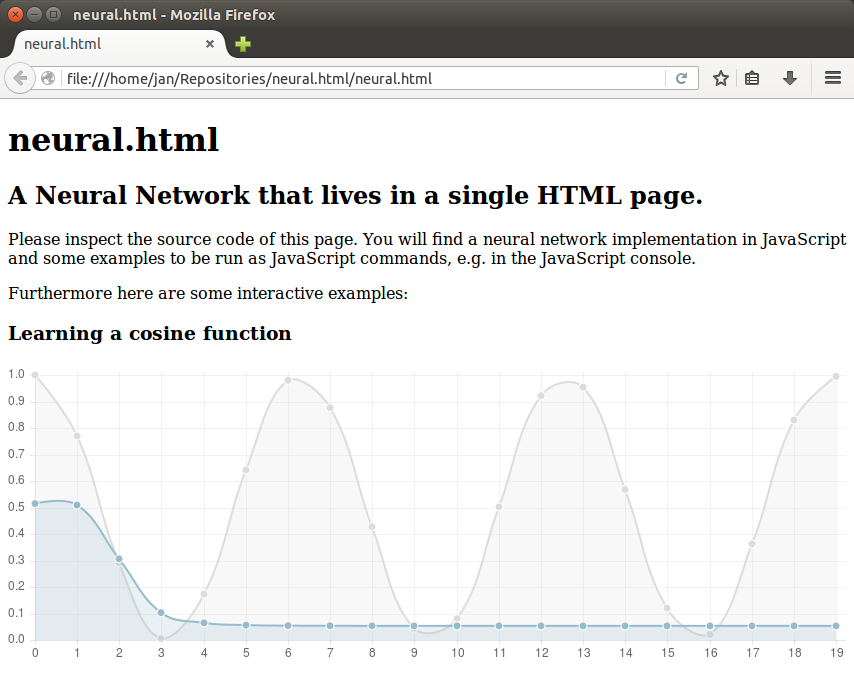
\includegraphics[width=0.9\textwidth]{screenshot.png}
  \end{figure}
}

\frame{
  \resizebox{0.2\linewidth}{!}{Thank you!}
}

\end{document}
